\section{Gustavo}

\setbeamertemplate{caption}{\raggedright\insertcaption\par}
\begin{frame}{Introduction}{Gustavo S. Buschle\newline<gbusch14@student.aau.dk>}
    \begin{figure}[h!]
        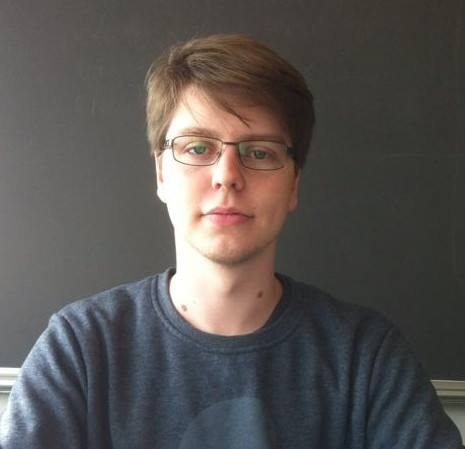
\includegraphics[width=0.3\textwidth]{images/gustavo.jpg}
        \caption{Gustavo S. Buschle}
        \centering
    \end{figure}
\end{frame}
\setbeamertemplate{caption}[default]

\begin{frame}{The Laser}{Gustavo S. Buschle\newline<gbusch14@student.aau.dk>}
    \begin{itemize}
        %probably split into more frames
        \item <1-> Assembly of Parts (pics)
        \item <2-> Two versions of the laser
        \item <3-> v1 with aduino: hard to sync
        \item <4-> v2 without arduino: slow
    \end{itemize}
\end{frame}

\begin{frame}{ROS}{Gustavo S. Buschle\newline<gbusch14@student.aau.dk>}
    \begin{itemize}
        \item <1-> Learning Curve
        \item <2-> ROS components we used
    \end{itemize}
\end{frame}

\begin{frame}{SLAM}{Gustavo S. Buschle\newline<gbusch14@student.aau.dk>}
    \begin{itemize}
        \item <1-> We didn't actually use it completely(pics)
        \item <2-> (linux time problems?)
    \end{itemize}
\end{frame}
